%To generate pdf:
%pdflatex description.tex

\documentclass{article}

\usepackage[letterpaper, margin=0.5in, footskip=2ex]{geometry}
\usepackage{graphicx} % Required to insert images
\usepackage{float} % For placing figures EXACTLY where I say
\usepackage{epstopdf}
\usepackage{listings} % Required for insertion of code
\usepackage{amssymb,amsmath}
%%\usepackage[open, openlevel=2]{bookmark}
\usepackage[hidelinks=true,bookmarks=true,bookmarksopen=true]{hyperref}

\graphicspath{ {fig_pdf/} } %If additional directories are needed, place them in additional sets of inner braces e.g {fig_pdf/}{fig_svg/}

\setlength{\parindent}{0pt}
\setlength{\parskip}{1ex}

\begin{document}

\title{Problem Description for Diffusion Through Nanopore}
\author{Tom Pace}
\maketitle

%%\tableofcontents

%-------------------------------------------------------------------------------
\section{Background}\label{sec:background}

We study a silica membrane containing nanoscopic circular pores arranged in a two-dimensional lattice.
We desire to understand the rate of transport of different ions through the nanopores,
quantified in terms of an effective diffusion constant.
The pore geometry is variable, as is the diffusion equation governing transport.
The diffusion equation is solved using \texttt{FEniCS}.

%-------------------------------------------------------------------------------
\section{System Geometry}\label{sec:geometry}

We study both a body-centered rectangular lattice of pores,
as well as a face-centered lattice of pores.
The unit cell geometry has two planes of symmetry.
This symmetry is used to reduce the model to only one quarter of the unit cell.

The body-centered geometry is shown in Figure \ref{fig:body-intro}.
The face-centered geometry is shown in Figure \ref{fig:face-intro}.

\begin{figure}[H]
\centering
\includegraphics[width=1\textwidth]{body-intro.pdf}
\caption{Body-centered geometry}
\label{fig:body-intro}
\end{figure}

\begin{figure}[H]
\centering
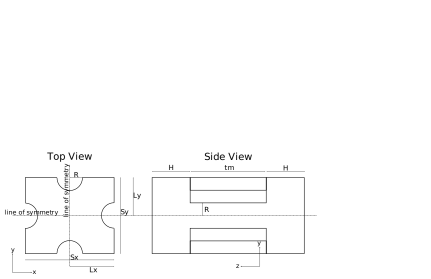
\includegraphics[width=1\textwidth]{face-intro.pdf}
\caption{Face-centered geometry}
\label{fig:face-intro}
\end{figure}

The geometric variables are:

$\begin{array}{rcl}
Sx & = & 2 Lx =\text{Unit cell x-dimension} \\
Sy & = & 2 Ly =\text{Unit cell y-dimension} \\
Lx & = & \frac{Sx}{2} =\text{Model x-dimension} \\
Ly & = & \frac{Sy}{2} =\text{Model y-dimension} \\
R & = & \text{Pore radius} \\
tm & = & \text{Membrane thickness} = \text{Pore length} \\
H & = & \text{Distance from membrane surface to model boundary}
\end{array}$

%-------------------------------------------------------------------------------
\section{Mesh Generation}\label{sec:meshgen}

\texttt{gmsh} is used to generate the finite element mesh.
The mesh is generated from solid geometry defined by its boundary surfaces.
These surfaces, in turn, are defined by their boundaries,
which are defined using points.

\textbf{TODO: gmsh geometry (point numbers, etc)}

%-------------------------------------------------------------------------------
\section{Result Calculations}

\subsection{Diffusion Constant}\label{subsec:D_eff}

To compute the equivalent diffusion constant, the problem is treated as a one-dimensional diffusion problem.
That is, we consider diffusion in the direction across the membrane.
The Fickian diffusion equation (see Section \ref{subsec:unhom_fick}) in one dimension is

$$j = - D_{\text{bulk}} \frac{dc}{ds}$$

where:

$\begin{array}{rcl}
s & = & \text{position within the one-dimensional domain} \\
j & = & j(s) = \text{flux at any point, in units of number of particles per unit area per unit time} \\
D_{\text{bulk}} & = & \text{diffusion constant of the medium, in units of area per unit time} \\
c & = & c(s) = \text{concentration at any point, in units of number of particles per unit volume} \\
\frac{dc}{ds} & = & \text{first spatial derivative of concentration}
\end{array}$

The three-dimensional problem is converted to an equivalent one-dimensional problem
by integrating over the area of the unit cell, in the two directions perpendicular to
the one-dimensional diffusion problem.
The total flux across the membrane will be given by:

$$J_{\text{cell}} = - D_{\text{bulk}}\int_{\text{cell}} dA\, \frac{\partial c}{\partial s}$$

We define the effective diffusion constant such that the integrated flux is the same,
when used with an the average concentration gradient across the membrane:

$$J_{\text{cell}} = - D_{\text{eff}} A_{\text{cell}} \frac{\Delta c}{\Delta s}$$

where:

$\begin{array}{rcl}
J_{\text{cell}} & = & \text{integral of flux over the pore, in units of number of particles per unit time} \\
A_{\text{cell}} & = & \text{area of unit cell} \\
D_{\text{eff}} & = & \text{unknown effective diffusion constant} \\
\Delta c & = & \text{change in concentration} \\
\Delta s & = & \text{distance over which concentration changes}
\end{array}$

Re-arranging this equation to solve for the unknown $D_{\text{eff}}$, we have:

$$D_{\text{eff}} = - \frac{J_{\text{cell}}}{A_{\text{cell}}} \frac{\Delta s}{\Delta c}$$

The integrated flux, $J_{\text{model}}$, is calculated from the model by integrating
the ion flux over a surface parallel to the membrane surface.
The result should be the same for any such surface capturing the full extents of the model.
That is, the integrated flux should be the same when integrating over the model pore as
when integrating over the upgradient or downgradient boundary of the model.

Specifically, the integrated flux is calculated as:

$$J_{\text{model}} = \int_{\text{model}} dA\, \left(\hat{n} \cdot \vec{j} \right)
 = - D_{\text{bulk}} \int_{\text{model}} dA\, \left(\hat{n} \cdot \vec{\nabla} c \right)$$

where $\hat{n}$ is the directed normal to the surface,
and $c$ is the concentration field found by solving the model.

Because of the use of planes of symmetry (see Section \ref{sec:geometry}),
the flux obtained by integration is only one quarter of the total for the unit cell.
That is, $J_{\text{cell}} = 4 J_{\text{model}}$.
With $A_{\text{cell}} = 4 Lx Ly$, we have:

$$D_{\text{eff}} = - \frac{4 J_{\text{model}}}{4 Lx Ly} \frac{\Delta s}{\Delta c}
 = - \frac{J_{\text{model}}}{Lx Ly} \frac{\Delta s}{\Delta c}$$

For convenience, we define the integral

$$I_{\text{gc}} = \int_{\text{model}} dA\, \left(\hat{n} \cdot \vec{\nabla} c \right)$$

then the flux integral is simply

$$J_{\text{model}} = - D_{\text{bulk}} I_\text{gc}$$

and the effective diffusion constant is

$$D_{\text{eff}} = D_{\text{bulk}} \frac{I_\text{gc}}{Lx Ly} \frac{\Delta s}{\Delta c}$$

This can also be written as

$$\frac{D_{\text{eff}}}{D_{\text{bulk}}} = \frac{I_\text{gc}}{Lx Ly} \frac{\Delta s}{\Delta c}$$

The values of $\Delta c$ and $\Delta s$ are calculated by extracting
the concentration result at two points located symmetrically on opposite sides of the membrane.
The difference in concentration between these two points is $\Delta c$,
and the distance between them is $\Delta s$.

Slightly different results for the value of $D_{\text{eff}}$ could be attained by selecting different
pairs of symmetrically located points.
For consistency, the results here are taken with these two points located
along the centerline of the pore, at both faces of the membrane.

\subsection{Free Volume Fraction}\label{subsec:volfrac}

The free volume fraction, $\phi$ is defined here as

$$\phi = \frac{\text{pore area}}{\text{unit cell area}}
= \frac{\pi R^2}{Sx Sy} = \frac{\pi R^2}{4 Lx Ly}$$

%-------------------------------------------------------------------------------
\section{Diffusion Equation}\label{sec:equation}

\subsection{Unhomogenized Fickian Diffusion Equation}\label{subsec:unhom_fick}

For particle flux defined as 

$$\vec{j} = - D_{\text{bulk}} \vec{\nabla} c$$

The Fickian diffusion equation can be written:
$$\frac{\partial c}{\partial t} = - \vec{\nabla} \cdot \vec{j}$$

where:

$\begin{array}{rcl}
c & = & c(x,y,z) = \text{the particle concentration field (number of particles per unit volume)} \\
t & = & \text{time} \\
\vec{j} & = & \vec{j}(x,y,z) = \text{the particle flux field (number of particles per unit area per unit time)} \\
D & = & \text{the implicit diffusion constant of the solvent (unit area per unit time)}
\end{array}$

For constant $D_{\text{bulk}}$, this can be written as

$$\frac{\partial c}{\partial t} = D_{\text{bulk}} \nabla^2 c$$

We seek the solution at equilibrium, defined by
$\frac{\partial c}{\partial t} = 0$ at all points in the problem domain.
Thus, we seek to solve

$$D_{\text{bulk}} \nabla^2 c = 0$$

subject to boundary conditions.

Assuming $D_{\text{bulk}}$ is any nonzero constant, this is clearly the same as

$$ \nabla^2 c = 0$$

For solution in \texttt{FEniCS}, a weak form of this equation is required.
Multiplying by a test function $v$ and integrating over the problem domain,

$$\int_{\Omega} \left(\nabla^2 c \right) v \,d^3x = 0$$

Using the product rule
$$\vec{\nabla} \cdot \left( v \vec{\nabla} c \right) =
v \left(\vec{\nabla} \cdot \vec{\nabla} c \right) + \vec{\nabla}c \cdot \vec{\nabla}v =
v \left(\nabla^2 c \right) + \vec{\nabla}c \cdot \vec{\nabla}v$$
$$\left(\nabla^2 c \right) v =
\vec{\nabla} \cdot \left( v \vec{\nabla} c \right) - \vec{\nabla}c \cdot \vec{\nabla}v$$

to integrate by parts, the equation becomes
$$ \int_{\Omega} \left(\nabla^2 c \right) v \,d^3x =
\int_{\Omega} \vec{\nabla} \cdot \left( v \vec{\nabla} c \right) \,d^3x
- \int_{\Omega} \left( \vec{\nabla}c \cdot \vec{\nabla}v \right) \,d^3x =0$$

Applying the divergence theorem (Gauss's theorem):
$$\int_{\partial\Omega} \left( \hat{n} \cdot \vec{\nabla} c \right) v\,ds
- \int_{\Omega} \left( \vec{\nabla}c \cdot \vec{\nabla}v \right) \,d^3x = 0$$

$$\int_{\Omega} \left( \vec{\nabla}c \cdot \vec{\nabla}v \right) \,d^3x =
\int_{\partial\Omega} \left( \hat{n} \cdot \vec{\nabla} c \right) v\,ds$$

In this case, we have both Dirichlet and von Neumann boundary conditions:
there are some boundary surfaces where the concentration is known,
and others where the particle flux is known.
Specifically, known concentrations are applied at both the top and bottom of the model,
and the particle flux must be zero for all other boundary surfaces.
Defining $\Gamma_D$ as the Dirichlet boundary surfaces,
and $\Gamma_N$ as the von Neumann boundary surfaces, we obtain

$$\int_{\Omega} \left( \vec{\nabla}c \cdot \vec{\nabla}v \right) \,d^3x =
\int_{\Gamma_D} \left( \hat{n} \cdot \vec{\nabla} c \right) v\,ds
+\int_{\Gamma_N} \left( \hat{n} \cdot \vec{\nabla} c \right) v\,ds$$

For the Dirichlet boundary surfaces (where the concentration is known),
the test function $v$ must be equal to zero,
as the variation of the unknown function must be zero at points where the function is known.

Furthermore, a flux of zero requires that the derivative of the concentration in a direction
normal to the boundary surface is zero.
That is, $\hat{n} \cdot \vec{\nabla} c = 0$ at all points on the von Neumann boundaries.

Therefore, the governing equation is simply
$$\int_{\Omega} \left( \vec{\nabla}c \cdot \vec{\nabla}v \right) \,d^3x = 0$$

In terms of \texttt{FEniCS}, this means that the bilinear form is
$a(c,v)=\left( \vec{\nabla}c \cdot \vec{\nabla}v \right) \,d^3x$,
and the linear form is constant, zero.

\subsection{Homogenized Fickian Diffusion Equation}\label{subsec:hom_fick}

\textbf{TODO}

\end{document}
